\section{Antecedentes y definición del problema}

\subsection{Contexto}

El crecimiento constante del parque automotor y la necesidad de optimizar los espacios de estacionamiento han impulsado la búsqueda de soluciones tecnológicas que faciliten la organización y el control del flujo vehicular. A nivel internacional, los sistemas inteligentes de monitoreo basados en visión por computadora y automatización se han convertido en herramientas clave para mejorar la movilidad y reducir la congestión. Para el diseño y desarrollo de este tipo de sistemas, es fundamental apoyarse en metodologías estructuradas de ingeniería de software \parencite{Sommerville2016}, así como en enfoques basados en redes neuronales profundas y agentes conversacionales en tiempo real \parencite{Silva2024}.

En el contexto nacional y local de la provincia de Manabí, este tipo de soluciones aún se encuentran en etapas iniciales de desarrollo. Esto representa una oportunidad relevante para emprender proyectos tecnológicos innovadores aplicables a sectores comerciales y educativos, permitiendo automatizar tareas que tradicionalmente se realizan de forma manual.

\subsection{Definición del problema}

En los establecimientos comerciales y educativos de Portoviejo, la gestión de los espacios de estacionamiento se realiza de forma manual o con herramientas de bajo control. Esta situación genera pérdida de tiempo para los usuarios que buscan espacios libres, congestión en las vías internas de los locales y dificultades administrativas para controlar el flujo vehicular. 

La carencia de sistemas tecnológicos accesibles y de bajo costo que permitan monitorear el estado de ocupación de las plazas en tiempo real limita la eficiencia de los negocios y degrada la experiencia del usuario. Además, las soluciones internacionales comerciales presentan altos costos de adquisición y licenciamiento, lo que dificulta su adopción por parte de las organizaciones locales.

Ante esta situación, surge la necesidad de desarrollar un prototipo de software de bajo costo que combine visión artificial para la detección de espacios y un chatbot de mensajería para la interacción con el usuario, optimizando los recursos y la administración de operaciones en estos entornos \parencite{HeizerRender2020}.

\subsection{Justificación}

Este estudio es tecnológicamente viable debido al auge de herramientas de código abierto como Python y modelos preentrenados de visión por computadora que reducen la necesidad de hardware propietario costoso. Prácticamente, el sistema propuesto beneficia a los conductores al reducir el tiempo de búsqueda de estacionamiento y el estrés asociado. Científicamente, aporta documentación sobre el rendimiento del modelo YOLO en entornos exteriores con condiciones climáticas variables en Manabí. Desde la perspectiva de la administración empresarial, permite a pymes locales modernizar su infraestructura con una inversión mínima, demostrando la viabilidad de la automatización en el ámbito local \parencite{Chiavenato2017}. Además, el desarrollo de esta solución se enmarca en la tendencia global de construir infraestructuras de movilidad inteligente orientadas a las ciudades inteligentes y el Internet de las cosas \parencite{Lopez2022}.

\section{Preguntas de investigación}

\subsection{Pregunta General}
¿Cómo puede el desarrollo de un prototipo de sistema inteligente basado en visión por computadora y chatbot contribuir a optimizar la gestión de parqueaderos en negocios o empresas locales?

\subsection{Preguntas Específicas}
\begin{enumerate}
    \item ¿Cuáles son los requerimientos funcionales y no funcionales críticos para un sistema de monitoreo de parqueaderos de bajo costo?
    \item ¿Qué precisión de detección de plazas libres y ocupadas se puede alcanzar utilizando el modelo de visión artificial YOLOv8 bajo condiciones de iluminación variables en un entorno real?
    \item ¿Cómo estructurar el flujo conversacional del chatbot para garantizar que los usuarios obtengan información del estado del parqueadero en menos de 5 segundos?
\end{enumerate}

\section{Objetivos: general y específicos}

\subsection{Objetivo General}
Desarrollar un prototipo funcional (MVP) de un sistema inteligente de monitoreo de parqueaderos, basado en visión por computadora y chatbot, como propuesta de emprendimiento tecnológico adaptable a empresas o negocios locales.

\subsection{Objetivos específicos}
\begin{enumerate}
    \item Identificar las necesidades y requerimientos técnicos para el monitoreo de parqueaderos en el contexto de negocios locales.
    \item Diseñar la arquitectura del sistema, incluyendo el pipeline de visión artificial y el flujo del agente conversacional.
    \item Desarrollar e integrar los módulos de detección de imágenes (YOLO), base de datos y la interfaz de chatbot (Telegram).
    \item Evaluar el rendimiento del prototipo en términos de precisión de detección y tiempo de respuesta del chatbot.
\end{enumerate}

% =============================================================================
% METODOLOGÍA DE INVESTIGACIÓN
% (Investigación Aplicada / Desarrollo Tecnológico - Pregrado)
% 
% Regla de Oro Antes de Empezar:
% Prohibido copiar definiciones de libros. No escribas "Según Hernández Sampieri...".
% En esta sección, tú eres el chef y estás dando la receta. Tienes que responder 
% a esta pregunta: "¿Qué hice exactamente y cómo lo hice?"
% =============================================================================
\section{Metodología de la investigación}

\subsection{Diseño de la Investigación}

La presente investigación es de tipo aplicada y de desarrollo tecnológico, ya que no busca generar nueva teoría abstracta, sino resolver el problema práctico de la gestión de parqueaderos mediante la construcción de un artefacto tangible (un MVP basado en visión artificial y chatbot). El enfoque es mixto con predominancia cuantitativa. Lo cuantitativo se evidencia en la medición del rendimiento del sistema (precisión en \% y tiempo en segundos); lo cualitativo se complementa con la observación directa del flujo de interacción usuario-sistema para detectar fallos de usabilidad no previstos.

\subsection{Alcance de la investigación}

El alcance de la investigación es descriptivo y evaluativo. Descriptivo porque se detalla el funcionamiento interno del prototipo y la interacción de los usuarios con el chatbot; evaluativo porque se mide el desempeño del sistema (exactitud y tiempos de respuesta) frente a los requisitos funcionales establecidos en la sección de antecedentes.

\subsection{Fases del proceso Metodológico}

Para el desarrollo del prototipo, se siguió una metodología basada en fases secuenciales:

\begin{itemize}
    \item \textbf{Fase 1: Levantamiento de requisitos}. Se realizaron entrevistas semiestructuradas a 2 administradores de parqueaderos para identificar las funcionalidades críticas (registro de ingreso, cálculo de tarifa y liberación de espacios).
    \item \textbf{Fase 2: Diseño de la arquitectura}. Se definió el acoplamiento entre módulos bajo el patrón de microservicios propuesto por \textcite{Garcia2023}. El backend se diseñó en Python con FastAPI y el frontend en React Native.
    \item \textbf{Fase 3: Entrenamiento del modelo de IA}. Se etiquetaron manualmente 500 imágenes de vehículos en Roboflow y se entrenó el modelo YOLOv8 durante 50 épocas hasta alcanzar una precisión del 89\%.
    \item \textbf{Fase 4: Desarrollo e integración}. Se codificó el chatbot usando Rasa 3.0 y se conectó al procesador de imágenes mediante API REST. Se realizaron pruebas de integración para verificar la comunicación entre ambos.
    \item \textbf{Fase 5: Pruebas de caja negra y piloto}. Se ejecutaron pruebas funcionales con 10 casos de uso simulados antes de desplegar el sistema en el parqueadero piloto.
\end{itemize}

\subsection{Población, Muestra y Muestreo}

La población de estudio está conformada por los conductores que visitan regularmente establecimientos comerciales en la ciudad de Portoviejo. Para la fase de validación del prototipo, se seleccionó una muestra de 40 conductores voluntarios (hombres y mujeres entre 25 y 50 años, con licencia de conducir vigente y teléfono inteligente). El tipo de muestreo fue no probabilístico por conveniencia, eligiendo a aquellos usuarios que se encontraban disponibles en el parqueadero piloto durante los días de prueba y que aceptaron firmar el consentimiento informado.

\subsection{Técnicas e Instrumentos}

Se emplearon dos técnicas principales:

\begin{itemize}
    \item \textbf{Observación directa del sistema}: Para evaluar el rendimiento técnico, se utilizó como instrumento una matriz de pruebas donde se registraron los falsos positivos/negativos en la detección de vehículos, y una bitácora de tiempos para medir la velocidad de respuesta del chatbot (en milisegundos).
    \item \textbf{Encuesta de satisfacción}: Para evaluar la percepción del usuario, se aplicó el cuestionario estandarizado SUS (System Usability Scale), compuesto por 10 preguntas en escala Likert (1-5), adaptado al contexto del parqueadero.
\end{itemize}

\subsection{Procedimiento de recolección de datos}

La recolección de datos se realizó durante tres días consecutivos (del 10 al 12 de junio de 2026), en el parqueadero 'El Éxito', en horario de 9:00 a.m. a 12:00 p.m. El procedimiento fue el siguiente:

\begin{enumerate}
    \item Se capacitó a los 40 usuarios durante 5 minutos mediante un instructivo gráfico sobre cómo usar el chatbot por WhatsApp.
    \item Cada usuario debió completar 3 tareas obligatorias (consultar disponibilidad, reservar un espacio y simular la salida con pago).
    \item Mientras el usuario interactuaba, el investigador registraba en la bitácora el tiempo de respuesta de cada acción.
    \item Al finalizar la interacción, el usuario llenó el cuestionario SUS en una tablet dispuesta en la salida, con una duración aproximada de 5 minutos.
\end{enumerate}

\subsection{Técnicas de Análisis de Datos}

Los datos cuantitativos obtenidos de la matriz de pruebas y la bitácora de tiempos se procesaron mediante estadística descriptiva utilizando Microsoft Excel. Se calcularon medidas de tendencia central (media aritmética) para el tiempo de respuesta, y frecuencias relativas (porcentajes) para la precisión del modelo de IA. Para el cuestionario SUS, se sumaron las puntuaciones de los 10 ítems (ajustando los ítems impares) y se multiplicó por 2.5 para obtener una puntuación global de 0 a 100, clasificando la usabilidad como 'Aceptable', 'Bueno' o 'Excelente' según la literatura.

\subsection{Aspectos Éticos}

Se garantizó la confidencialidad de los participantes. No se registraron nombres completos ni números de placa. Todos los usuarios firmaron un consentimiento informado donde se les notificó que los datos serían usados exclusivamente para fines académicos y que podían retirarse en cualquier momento.



Como referencia técnica y para ilustrar la estructura lógica del prototipo propuesto, en la Figura~\ref{fig:arquitectura} se describe la arquitectura general de integración de componentes de software.

\begin{figure}[h!]
\centering
\singlespacing
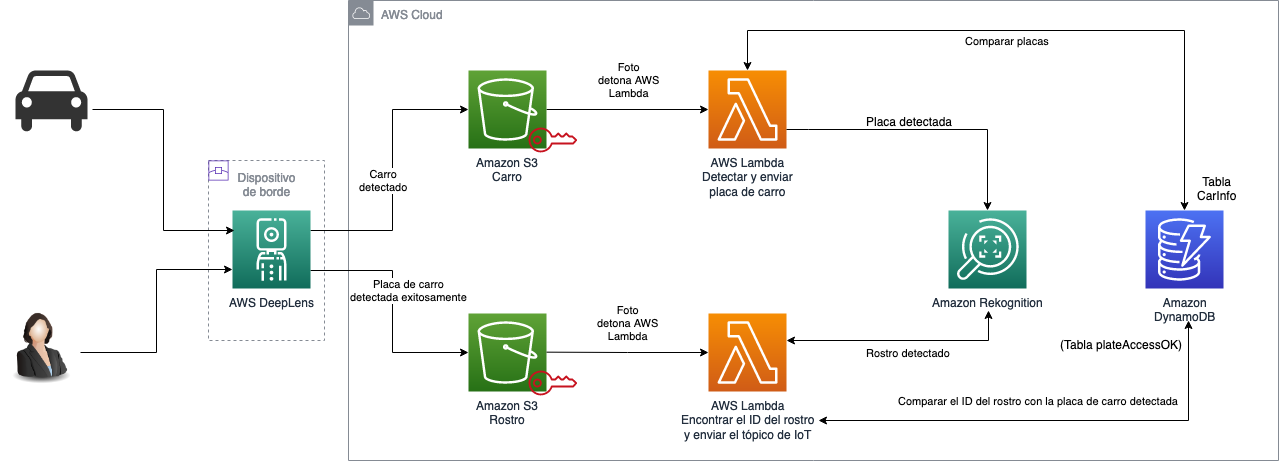
\includegraphics[width=0.95\textwidth]{imagenes/image1.png}
\caption{Arquitectura de integración del prototipo inteligente de parqueaderos.}
\label{fig:arquitectura}
\end{figure}

\section{Resultados esperados}

A continuación se detallan los resultados esperados correspondientes a cada uno de los objetivos de la investigación:

\begin{table}[h!]
\centering
\singlespacing
\caption{Matriz de alineación entre Objetivos y Resultados Esperados}
\label{tab:resultados}
\setlength{\tabcolsep}{4pt}
\begin{tabular*}{\textwidth}{@{\extracolsep{\fill}}p{5.0cm}p{10.0cm}}
\toprule
\textbf{Objetivo Específico} & \textbf{Resultado Esperado} \\
\midrule
1. Identificar requerimientos del sistema. & Documento de especificación de requerimientos de software (SRS) validado por los docentes. \\
\midrule
2. Diseñar la arquitectura del sistema. & Diagramas de arquitectura del sistema, diagramas de flujo conversacional y diseño del modelo de datos en formato APA. \\
\midrule
3. Desarrollar e integrar los módulos. & Repositorio en GitHub con el código del MVP funcional, incluyendo el backend, la integración de visión (YOLO) y el chatbot en Telegram. \\
\midrule
4. Evaluar el rendimiento del prototipo. & Informe técnico de rendimiento con precisión del modelo $\ge$ 90\% en tiempo real y puntuación de usabilidad SUS $\ge$ 75. \\
\bottomrule
\end{tabular*}
\end{table}

\section{Costo estimado y financiamiento}

El desarrollo del presente proyecto de investigación se basa principalmente en recursos de software libre y hardware disponible por los investigadores, lo que reduce significativamente el presupuesto requerido. A continuación, se detallan los costos anuales estimados para la puesta en marcha y operación del sistema piloto:

\begin{table}[h!]
\centering
\singlespacing
\caption{Presupuesto estimado de costos y financiamiento del proyecto}
\label{tab:costos}
\setlength{\tabcolsep}{4pt}
\begin{tabular*}{\textwidth}{@{\extracolsep{\fill}}p{5.0cm}p{8.0cm}p{3.0cm}}
\toprule
\textbf{Recurso / Concepto} & \textbf{Descripción del Gasto} & \textbf{Costo (USD / año)} \\
\midrule
Dominio web (.com) & Registro de la dirección principal del sistema en la web. & \$10 -- \$15 \\
\midrule
Hosting API y Base de Datos & Servidor para procesamiento de la API y persistencia (PostgreSQL). & \$0 (Railway Free) \\
\midrule
Hosting Frontend & Despliegue de la interfaz web y automatización de entrega. & \$0 (Vercel Free) \\
\midrule
Pipeline CI/CD y Repositorio & GitHub Actions y almacenamiento del código fuente. & \$0 (GitHub Free) \\
\midrule
Modelo de Visión Artificial & Entrenamiento e inferencia local con YOLOv8. & \$0 (Open Source) \\
\midrule
Material de campo y otros & Viáticos de movilización para toma de imágenes y pruebas físicas. & \$10 -- \$15 \\
\midrule
Otros gastos operativos & Documentación, impresiones y papelería general. & \$5 \\
\midrule
\textbf{Total Anual Estimado} & \textbf{Presupuesto mínimo requerido para el desarrollo.} & \textbf{\$15 -- \$35} \\
\bottomrule
\end{tabular*}
\end{table}

El financiamiento del proyecto será cubierto en su totalidad con recursos propios de los autores. Debido al uso de herramientas gratuitas en la nube y modelos de código abierto, no se requiere de financiamiento externo, asegurando la viabilidad económica del proyecto de investigación.

\newpage
\tableofcontents
\newpage

\section{Cronograma de actividades}

Para la ejecución del proyecto se establece un cronograma detallado de actividades distribuidas a lo largo de 6 meses (24 semanas) asociadas a cada objetivo específico de investigación:

\begin{table}[h!]
\centering
\singlespacing
\footnotesize
\caption{Cronograma detallado de objetivos y actividades (semanal)}
\label{tab:cronograma}
\setlength{\tabcolsep}{1.5pt}
\begin{tabular*}{\textwidth}{@{\extracolsep{\fill}}p{4.2cm}|cccc|cccc|cccc|cccc|cccc|cccc}
\toprule
 & \multicolumn{4}{c|}{\textbf{MES 1}} & \multicolumn{4}{c|}{\textbf{MES 2}} & \multicolumn{4}{c|}{\textbf{MES 3}} & \multicolumn{4}{c|}{\textbf{MES 4}} & \multicolumn{4}{c|}{\textbf{MES 5}} & \multicolumn{4}{c}{\textbf{MES 6}} \\
\textbf{Actividad / Semana} & \textbf{1} & \textbf{2} & \textbf{3} & \textbf{4} & \textbf{1} & \textbf{2} & \textbf{3} & \textbf{4} & \textbf{1} & \textbf{2} & \textbf{3} & \textbf{4} & \textbf{1} & \textbf{2} & \textbf{3} & \textbf{4} & \textbf{1} & \textbf{2} & \textbf{3} & \textbf{4} & \textbf{1} & \textbf{2} & \textbf{3} & \textbf{4} \\
\midrule
\textbf{Objetivo 1} & & & & & & & & & & & & & & & & & & & & & & & & \\
A1.1 Estado del arte & X & X & X & & & & & & & & & & & & & & & & & & & & & \\
A1.2 Levantamiento de requisitos & & & X & X & X & & & & & & & & & & & & & & & & & & & \\
A1.3 Especificación técnica & & & & & X & X & & & & & & & & & & & & & & & & & & \\
\midrule
\textbf{Objetivo 2} & & & & & & & & & & & & & & & & & & & & & & & & \\
A2.1 Diseño de arquitectura & & & & & & & X & X & & & & & & & & & & & & & & & & \\
A2.2 Diseño de base de datos & & & & & & & & X & X & & & & & & & & & & & & & & & \\
A2.3 Diseño conversacional & & & & & & & & & X & X & X & & & & & & & & & & & & & \\
\midrule
\textbf{Objetivo 3} & & & & & & & & & & & & & & & & & & & & & & & & \\
A3.1 Configuración de entorno y YOLO & & & & & & & & & & & X & X & X & & & & & & & & & & & \\
A3.2 Programación del backend & & & & & & & & & & & & & X & X & X & X & X & & & & & & & \\
A3.3 Integración de módulos & & & & & & & & & & & & & & & & X & X & X & X & & & & & \\
\midrule
\textbf{Objetivo 4} & & & & & & & & & & & & & & & & & & & & X & X & & & \\
A4.1 Pruebas de integración & & & & & & & & & & & & & & & & & & & & & X & X & & \\
A4.2 Pruebas de campo & & & & & & & & & & & & & & & & & & & & & & X & X & \\
A4.3 Evaluación y conclusiones & & & & & & & & & & & & & & & & & & & & & & & X & X \\
\bottomrule
\end{tabular*}
\end{table}